\documentclass[journal,12pt,twocolumn]{IEEEtran}

\usepackage{setspace}
\usepackage{gensymb}
\singlespacing
\usepackage[cmex10]{amsmath}

\usepackage{amsthm}
\usepackage{amsmath} 

\usepackage{mathrsfs}
\usepackage{txfonts}
\usepackage{stfloats}
\usepackage{bm}
\usepackage{cite}
\usepackage{cases}
\usepackage{subfig}

\usepackage{longtable}
\usepackage{multirow}

\usepackage{enumitem}
\usepackage{mathtools}
\usepackage{steinmetz}
\usepackage{tikz}
\usepackage{circuitikz}
\usepackage{verbatim}
\usepackage{tfrupee}
\usepackage[breaklinks=true]{hyperref}
\usepackage{graphicx}
\usepackage{tkz-euclide}

\usetikzlibrary{calc,math}
\usepackage{listings}
    \usepackage{color}                                            %%
    \usepackage{array}                                            %%
    \usepackage{longtable}                                        %%
    \usepackage{calc}                                             %%
    \usepackage{multirow}                                         %%
    \usepackage{hhline}                                           %%
    \usepackage{ifthen}                                           %%
    \usepackage{lscape}     
\usepackage{multicol}
\usepackage{chngcntr}

\DeclareMathOperator*{\Res}{Res}

\renewcommand\thesection{\arabic{section}}
\renewcommand\thesubsection{\thesection.\arabic{subsection}}
\renewcommand\thesubsubsection{\thesubsection.\arabic{subsubsection}}

\renewcommand\thesectiondis{\arabic{section}}
\renewcommand\thesubsectiondis{\thesectiondis.\arabic{subsection}}
\renewcommand\thesubsubsectiondis{\thesubsectiondis.\arabic{subsubsection}}


\hyphenation{op-tical net-works semi-conduc-tor}
\def\inputGnumericTable{}                                 %%

\lstset{
%language=C,
frame=single, 
breaklines=true,
columns=fullflexible
}
\begin{document}


\newtheorem{theorem}{Theorem}[section]
\newtheorem{problem}{Problem}
\newtheorem{proposition}{Proposition}[section]
\newtheorem{lemma}{Lemma}[section]
\newtheorem{corollary}[theorem]{Corollary}
\newtheorem{example}{Example}[section]
\newtheorem{definition}[problem]{Definition}

\newcommand{\BEQA}{\begin{eqnarray}}
\newcommand{\EEQA}{\end{eqnarray}}
\newcommand{\define}{\stackrel{\triangle}{=}}
\bibliographystyle{IEEEtran}
\raggedbottom
\setlength{\parindent}{0pt}
\providecommand{\mbf}{\mathbf}
\providecommand{\pr}[1]{\ensuremath{\Pr\left(#1\right)}}
\providecommand{\qfunc}[1]{\ensuremath{Q\left(#1\right)}}
\providecommand{\sbrak}[1]{\ensuremath{{}\left[#1\right]}}
\providecommand{\lsbrak}[1]{\ensuremath{{}\left[#1\right.}}
\providecommand{\rsbrak}[1]{\ensuremath{{}\left.#1\right]}}
\providecommand{\brak}[1]{\ensuremath{\left(#1\right)}}
\providecommand{\lbrak}[1]{\ensuremath{\left(#1\right.}}
\providecommand{\rbrak}[1]{\ensuremath{\left.#1\right)}}
\providecommand{\cbrak}[1]{\ensuremath{\left\{#1\right\}}}
\providecommand{\lcbrak}[1]{\ensuremath{\left\{#1\right.}}
\providecommand{\rcbrak}[1]{\ensuremath{\left.#1\right\}}}
\theoremstyle{remark}
\newtheorem{rem}{Remark}
\newcommand{\sgn}{\mathop{\mathrm{sgn}}}
\providecommand{\abs}[1]{\left\vert#1\right\vert}
\providecommand{\res}[1]{\Res\displaylimits_{#1}} 
\providecommand{\norm}[1]{\left\lVert#1\right\rVert}
%\providecommand{\norm}[1]{\lVert#1\rVert}
\providecommand{\mtx}[1]{\mathbf{#1}}
\providecommand{\mean}[1]{E\left[ #1 \right]}
\providecommand{\fourier}{\overset{\mathcal{F}}{ \rightleftharpoons}}
%\providecommand{\hilbert}{\overset{\mathcal{H}}{ \rightleftharpoons}}
\providecommand{\system}{\overset{\mathcal{H}}{ \longleftrightarrow}}
	%\newcommand{\solution}[2]{\textbf{Solution:}{#1}}
\newcommand{\solution}{\noindent \textbf{Solution: }}
\newcommand{\cosec}{\,\text{cosec}\,}
\providecommand{\dec}[2]{\ensuremath{\overset{#1}{\underset{#2}{\gtrless}}}}
\newcommand{\myvec}[1]{\ensuremath{\begin{pmatrix}#1\end{pmatrix}}}
\newcommand{\mydet}[1]{\ensuremath{\begin{vmatrix}#1\end{vmatrix}}}
\numberwithin{equation}{subsection}
\makeatletter
\@addtoreset{figure}{problem}
\makeatother
\let\StandardTheFigure\thefigure
\let\vec\mathbf
\renewcommand{\thefigure}{\theproblem}
\def\putbox#1#2#3{\makebox[0in][l]{\makebox[#1][l]{}\raisebox{\baselineskip}[0in][0in]{\raisebox{#2}[0in][0in]{#3}}}}
     \def\rightbox#1{\makebox[0in][r]{#1}}
     \def\centbox#1{\makebox[0in]{#1}}
     \def\topbox#1{\raisebox{-\baselineskip}[0in][0in]{#1}}
     \def\midbox#1{\raisebox{-0.5\baselineskip}[0in][0in]{#1}}
\vspace{3cm}
\title{Assignment 1}
\author{BILLAKURTHI SHAI SASI DEEP \\ SM21MTECH12006}
\maketitle
\newpage
\bigskip
\renewcommand{\thefigure}{\theenumi}
\renewcommand{\thetable}{\theenumi}
\section{Problem IV (4\Large{ii})}
\\Show that the following triad of points form an equilateral triangle \myvec{a\\0}, \myvec{0\\2a}, \myvec{2a\\a}, axes being inclined at an angle of 60$^{\circ}$
\subsection{Solution}
Let the points be
\begin{equation}
\myvec{x_1\\y_1} = \myvec{a \\0}  ; \myvec{x_2\\y_2}  = \myvec{0\\ 2a}; \myvec{x_3\\y_3} =  \myvec{2a \\a}\label{1.0.1} 
\end{equation}
In order to convert to rectangular coordinate system, the y-axis should be rotated by $30^{\circ}$ in anti-clockwise.
Transformed coordinates of \myvec{x_1\\y_1}, \myvec{x_2\\y_2} \& \myvec{x_3\\y_3} be \myvec{x_4\\y_4}, \myvec{x_5\\y_5} \& \myvec{x_6\\y_6} respectively.\\\\
$x_4$ = O$X_1$ + $X_1$$X_4$ = $x_1$+$y_1$$\cos{60^{\circ}$\\
$y_4$ = O$Y_1$$\cos{30^{\circ}$$ = $y_1$$\cos{30^{\circ}$\\
\begin{equation}
\myvec{x_4\\y_4} = \myvec{1 \ \cos{60^{\circ}} \\ 0 \  \cos{30^{\circ}}} \myvec{x_1\\y_1}\label{eq:1.0.2}   
\end{equation}
The generalised equation for transformed coordinates $\myvec{x_t\\y_t}$ when the angle between axes `$\theta$ is,
\begin{equation}
\boxed{\myvec{x_t\\y_t} = \myvec{1   \ \  \cos{(\theta)} \\ 0 \ \ \sin{(\theta)}} \myvec{x\\y}} \label{eq:1.0.3}  
\end{equation}
Let the transformed point be $\vec{X_t}$, $\vec{T}$ be the transformation matrix and the point in angular axes be $\vec{X}$, \eqref{eq:1.0.3} can be written as 
\begin{equation}
 \vec{X_t} = \vec{T} \ \vec{X}\label{eq:1.1.5}  
\end{equation}
Substituting \eqref{1.0.1} in \eqref{eq:1.0.3} 
 \begin{equation}
  \myvec{x_4\\y_4} = \myvec{a\\0};\ \myvec{x_5\\y_5} = \myvec{a\\\sqrt{3}a};\myvec{x_6\\y_6} =\myvec{\frac{5a}{2}\\\frac{\sqrt{3}a}{2}} \label{eq:1.0.5}    
 \end{equation}
The distance between points is a norm of the distance vector,
\begin{equation}
d_{12} = \norm{\vec{X_t_1}-\vec{X_t_2}} \label{eq:1.1.7}
\end{equation}
Substituting \eqref{eq:1.1.5} in \eqref{eq:1.1.7},
\begin{equation}
d_{12} = \norm{\vec{T}\vec{X_1}-\vec{T}\vec{X_2}} \label{eq:1.1.8}
\end{equation}
\begin{equation}
d_{12} = \norm{\vec{T}(\vec{X_1}-\vec{X_2})} \label{eq:1.1.123}
\end{equation}
\begin{equation}
d_{12}= (\vec{X_1}-\vec{X_2})^\top \  \vec{T}^\top \  \vec{T} \ (\vec{X_1}-\vec{X_2})  \label{eq:1.1.9}
\end{equation}
\begin{align}
d_{12} = \sqrt{3}a \\
similarly,    d_{23}=\sqrt{3}a \\
d_{31}=\sqrt{3}a 
\end{align}
Therefore,
\begin{equation}
    d_{12}=d_{23}=d_{31}    \label{eq:1.1.13}
\end{equation}
From \eqref{eq:1.1.13} 
The three points form equilateral triangle
\counterwithin{figure}{section}
\begin{figure}[!ht]
	\centering
	\includegraphics[width=\columnwidth]{BOP1.jpg}
	\caption{Points defined on angular \& rectangular axes}
	\end{figure}
\counterwithin{figure}{section}
\begin{figure}[!ht]
    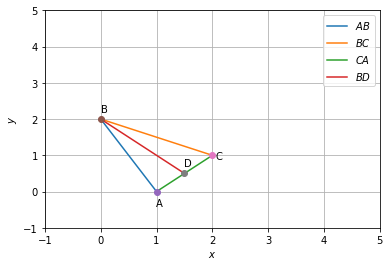
\includegraphics[width=\columnwidth]{tri.png}
    \caption{Points plotted in Python}
    \label{Fig2: Points plotted in Python}
\end{figure}

\end{document}